\documentclass[a4paper,12pt]{article}

% Packages
\usepackage{graphicx}
\usepackage{amsmath}
\usepackage{geometry}
\usepackage{fancyhdr}
\usepackage{setspace}
\usepackage{titlesec}  % For title formatting
\geometry{margin=1in}
\setstretch{1.5}
\usepackage{url}

% Header and Footer
\pagestyle{fancy}
\fancyhf{}
\fancyhead[L]{Newtons avkjølings lov}
\fancyhead[R]{\thepage}

% Title Formatting
\titleformat{\section}{\normalfont\Large\bfseries}{\thesection}{1em}{}

% Cover Page
\title{
    \vspace{2cm} % Adjust vertical space
    
\includegraphics[width=0.55\textwidth]{ntnu_hoeyde_eng.png} \\ % Add your logo here (change "logo.png" to the actual filename)
    \vspace{1cm} % Adjust vertical space after the logo
    \textbf{\Huge Newtons avkjølings lov} \\
    \vspace{1cm} % Adjust vertical space
    \large TMA4101 Matematikk 1 \\
    \vspace{0.5cm} % Adjust vertical space
    \large 11.11.2024
}
\author{Hallur Hermannsson Aspar \\ Jacob Mørk \\ Ola Brenno Søland \\ Erlend Dukefos Skretteberg \\ Erik Fransisco Valdeon Hauslo}
\renewcommand*\contentsname{Innhold}
\date{}

\begin{document}

% Title Page
\maketitle
\thispagestyle{empty}
\newpage

% Table of Contents
% Start page numbering from the Table of Contents
\setcounter{page}{1}  % Start counting from 1
\tableofcontents
\newpage

% 1. Objective or Summary
\section{Formål}
I dette forsøket ble Newtons avkjølingslov brukt til å finne
proporsjonalitetskonstanten til et glass med Pepsi Max (500 ml). \\
\[\ r = \frac{\--ln\left(\frac{5}{11}\right)}{60} \]


\section{Teori}
En kan sette opp en lineær modell for temperatur hvor en har tid på x-aksen og temperatur på y-aksen, og en konstant som endres for å ta hensyn til objekter sine egenskaper. 
\[T(t)=k*x\] 
Her setter vi konstanten til \(k=1\) fordi det blir lettere å regne med. Vi setter opp et eksempel med denne k-en: 
En is på -5 grader som smelter til vann med en temperatur på 10 grader i løpet av en tid på 15 minutter. Da kan en sette opp deltaY (temperaturendring i isen) over deltaX (endirng i tid) og regne temperaturendring i minuttet. 
\[\frac{10-(-5)}{15-0}=1\]\quad \\ 
Dette stemmer ikke helt med virkeligheten på grunn av to ting;  faseovergangen når isen smelter, og at forskjellen i temperatur mellom isen og omgivelsene blir mindre. Å smelte isen krever ekstra energi, fordi de intermolekylære kreftene som utgjør isens krystallstruktur må brytes for å kunne danne vann i væskeform. Den andre grunnen er at forskjellen i temperatur mellom isen og omgivelsene blir mindre. Derfor vil temperaturendringen avta helt til isen er samme temperatur som omgivelsene. \\
\\
Derfor fungerer ikke en lineær modell, og vi må ty til en differensiallikning. Denne differensiallikningen må ta hensyn til hvor fort temperaturen endres, objektenes egenskaper, temperaturen nå og temperaturen i omgivelsene. Dette har Isaac Newton allerede tenkt på med sin avkjølingslov.
\[\frac{Td}{dt}=-k(T-Tk)\]\quad \\
Hvor \(\frac{Td}{dt}\) er hvor fort temperaturen endres over tid, altså temperatur derrivert.\\
-k er en konstant som tar hensyn til objektet sin varmekapasitet og overflate.\\
T er temperaturen til objektet i forskjellige tidspunkter.\\ Tk er den konstante temperaturen til omgivelsene.\\
Dette gir oss en bedre modell av temperaturendringen til et objekt sammenliknet med den lineære modellen gitt som eksempel over.

% 2. Problem Description
\section{Eksperimentelt}
Dette forsøket var ganske enkelt å utføre. En Pepsi Max-boks, et termometer og et vanlig 500 mL glass ble brukt. Den kalde Pepsi Max-boksen ble åpnet og helt i glasset, og deretter ble termometeret satt oppi. Temperaturen ble målt med 15 minutters mellomrom til det hadde gått én time. Termometeret ble deretter rengjort og lagt i rommet en stund for å måle hvor varmt rommet var.

% 3. Methodology/Design Procedures
\section{Resultater}
Ved hjelp av målingene hvert 15. minutt, og romtemperatur, var det mulig å visualisere Newtons avkjølingslov med hjelp av Python. 
Grafen nedenfor viser temperaturendring over tid for innholdet i brusboksen, hvor de eksperimentelle datene er plottet i Python.
\\
Vi har gitt likningen:
\[16 = 21 + (10 - 21) e^{-r60}\]
Forenkle likningen:
\[16 = 21 - 11 e^{-r60}\]
Trekk 21 fra begge sider:
\[16 - 21 = -11 e^{-r60}\]
\[-5 = -11 e^{-r60}\]
Del begge sider med -11:
\[\frac{-5}{-11} = e^{-r60}\]
\[\frac{5}{11} = e^{-r60}\]
Ta den naturlige logaritmen (ln) på begge sider:
\[\-ln\left(\frac{5}{11}\right) = -60r\]
Vi deler på 60, og da får vi:
\[\ r = \frac{\--ln\left(\frac{5}{11}\right)}{60} \]

\newpage
\noindent\textbf{Ved å sette opp en python kode, vil man kunne fremstille avkjølingsloven og se temperaturendringen plottet som funksjon av tiden:} 

\begin{verbatim}

import numpy as np
import matplotlib.pyplot as plt

# Gitte verdier
T_omg = 21  # Omgivelsestemperatur i grader Celsius
T_0 = 10    # Starttemperatur i grader Celsius
k = -np.log(5/11)/60  # Avkjølingskonstant

# Tid i minutter
t = np.linspace(0, 120, 10000)  # Fra 0 til 60 minutter

# Newtons avkjølingslov
T_t = T_omg + (T_0 - T_omg) * np.exp(-k * t)

# Plotting
plt.figure(figsize=(8, 5))
plt.plot(t, T_t, label="Temperatur over tid", color="blue")
plt.xlabel("Tid (minutter)")
plt.ylabel("Temperatur (°C)")
plt.title("Oppvarming i henhold til Newtons avkjølingslov")
plt.grid(True)
plt.legend()
plt.show()
\end{verbatim}
\newpage

Som gir plottet:

\begin{figure}[h]
    \centering
    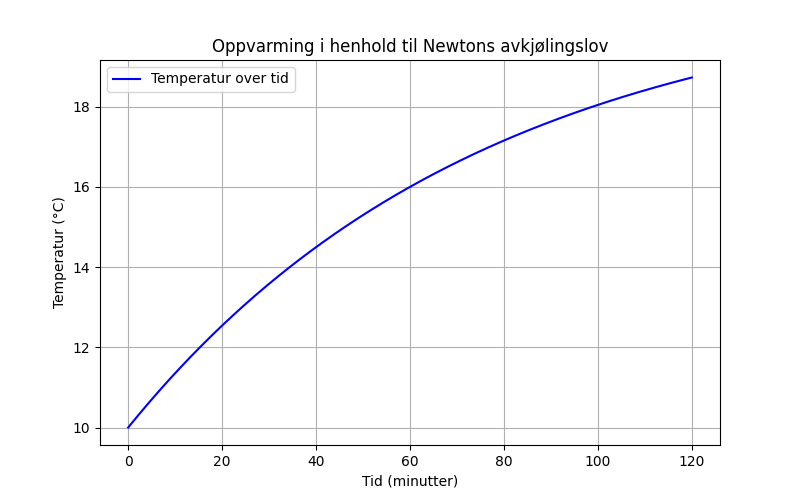
\includegraphics[width=1.0\linewidth]{Figure_1.png}
    
    \label{fig:Oppvarming i henhold til newtons avkjølingslov}
\end{figure}

Målingene som ble gjort hvert 15. minutt registrerte følgende temperaturer: 
\begin{itemize}
start = 10C
\\
15 min = 12C
\\
30 min = 13C
\\
45 min = 14C
\\
60 min = 16C
\\
75 min = 17C
\end{itemize}
Og man ser dermed at grafen gir et nokså riktig bilde av den faktiske oppvarmingen




4. Measurement/Testing Results
\newpage
\section{Diskusjon}
%Newtons avkjølingslov:
%\[\frac{Td}{dt}=-k(T-Tk)\]\quad  
Selv om grafen gir et ganske godt bilde av oppvarmingen, stemmer den ikke til punkt og prikke. \\

Generelt sett synker løseligheten til gasser i vann ved økende temperatur (Pedersen, 2023). Dette medfører at ulike gasser, særlig kullsyre og nitrogen, forlater væsken over tid når den varmes opp. Dette endrer væskens fysiske sammensetning og masse, og dermed minker løsningens varmekapasitet. Væskens volum vil også endres, og dermed endre væskens overflateareal. Dette påvirker hastigheten til varmeoverføring fra omgivelsene til brusen.\\

Oppløsning av kullsyre og nitrogen i vann er eksoterme prosesser, da vil den motsatte prosessen være endoterm. Dette vil si at det tas opp energi fra løsningen når kullsyre og nitrogen skal gå ut av løsning. Dette vil føre til en kjøle-effekt som vil sinke oppvarmingen.

Luftsirkulasjon vil også påvirke hvor fort varmen overføres. Ved lav luftsirkulasjon dannes det et tynt luftlag av stasjonær luft rundt objektet som kan gi en isolererende effekt. Ved høyere luftsirkulasjon vil denne effekten minimeres. Modellen tar ikke hensyn til dette.\\

Totalt sett er denne differsialligning en forenklet modell av virkeligheten, men i de fleste tilfeller er denne forenklingen mer enn god nok til å simulere virkeligheten. Flere av disse feilkildene som tapet av varmekapasitet fra gasstap og avkjøling fra den endoterme fysiske prosessen er uansett sannsynligvis så små at usikkerheten ved temperaturmåliing gir et større avvik fra modellen enn de utelatte faktorene.
\\
%skriv om andre ting som påvirker temperatur her (kullsyre som forsvinner, det er gass som forlater løsningen og endrer på varmekapasiteten)




%\begin{figure}[h!]
 %   \centering
  %  \includegraphics[width=0.8\textwidth]{example-image} % Example of adding a figure
    %\caption{Test results for circuit 1}
    %\label{fig:circuit1}
%\end{figure}

\newpage
% Bibliography (if required)
\bibliographystyle{plain}
\bibliography{references}  % Add a .bib file if you have references
\begin{itemize}
    \item Boyce, W.E., DiPrima, R.C. (1992). \textit{Elementary Differential Equations and Boundary Value Problems. John Wiley & Sons.}\\
Hentet 11.11.2024 fra: \url{https://www.nkhansen.com/tag/newtons-avkjolingslov/}

    \item Persen, B. (2023, 23. januar). Løsning (kjemi). I \textit{Store norske leksikon} \\
    \url{https://snl.no/.versionview/2445839}
    
\end{itemize}

\end{document}
